\chapter{Prerequisites}\label{ch:Theory}
The concepts used in this thesis require some prior knowledge about basic calculus and linear
algebra as well as some more advanced topics that will be introduced in the following sections.
Firstly, we will review some of the basic ideas that are needed to understand the rest of the
theory.
Afterwards, we explain the so called \textit{structure tensor} as well as the 
theory of diffusion and inpainting.
\section{Basics}\label{sec:Basics}
Before explaining corner detection and diffusion, we have to first define what an image is
mathematically.\\
A \textit{grey value image} is defined as a function $f: \Omega \rightarrow \R$ where
$\Omega \subset \R^2$ is a rectangular subset of $\R^2$ of size $n_x\times n_y$,
wheras a
\textit{colour image} is defined as a vector-valued function $f: \Omega \rightarrow \R^3$.
For the sake of simplicity, we will focus on grey value images as most of the results can easily be
transferred to vector-valued images.\\
\textbf{Notation:} Instead of writing $(x, y)$, we will use $\boldsymbol x := (x, y)$ most of the
time, as it makes most equations and definitions more readable. Furthermore, lowercase bold letters will denote vectors and uppercase bold letters will
denote matrices.
\subsection{Partial Derivatives}
One of the most important operations on functions in image processing is \textit{partial
    differentiation}.
The partial derivative of an image $f: \Omega \rightarrow \R$ in $x$-direction is herein denoted as $f_x$ or
synonymously as $\partial_x f$ and defined as
\begin{equation}
    f_x(x, y) = \partial_x f (x, y) = \frac{\partial f}{\partial x} (x, y) := \lim_{h \to 0}\frac{f(x+h, y) -f(x, y)}{h} 
\end{equation}
The \textit{gradient} of an image $f$ at position $(x, y)$ is the vector containing both partial
image derivatives at this position.\newpage\noindent
In multivariate calculus, the gradient of a function is an important tool to find the (both local
and global) extrema of a function similar to the first derivative for a function with a single
variable.
\begin{equation}
    \textbf{grad}(f) = \del f := {\left(f_x, f_y\right)}^\top\label{def:Grad}
\end{equation}
The gradient always points in the direction of the steepest ascent/descent, it is the tangent
vector to the surface at the given location~\cite{mfi3}. Furthermore, a vector that is
\textit{orthogonal} to the gradient always points into the direction of the smallest absolute
change at the given position.\\
Two vectors $x,y\in\R^n$ are called \textit{orthogonal} to each other if the Euclidean dot product defined by 
\begin{equation}\label{eq:EucDot}
    \langle\mathbf{x}, \mathbf{y}\rangle = \sum_{i=1}^n x_{i}y_i
\end{equation}
vanishes or, in other words, becomes zero.
The geometric interpretation for this property is that the angle between both vectors is 90°.

\subsection{Convolution}
Another operation from calculus that we will need is the \textit{convolution operator}.\\
\begin{equation}
    (f * g)(\boldsymbol x) := \int\limits_{\R^2} f(\boldsymbol x-\boldsymbol y)g(\boldsymbol y)d\boldsymbol y\label{eq:2DConv}
\end{equation}
The \textit{discrete} convolution of two vectors ${(f_i)}_{i\in\Z}, {(g_i)}_{i\in\Z}$ is usually defined as
\begin{equation}
    {(f*g)}_i := \sum_{j\in\Z} f_{i-j}g_i
\end{equation}
In both definitions, the function or vector $g$ is usually called the \textit{convolution kernel}.
In praxis though, discrete convolution has to be used as dealing with continuous functions in a
computational context is strictly not possible. This is why continuous convolution is only used to
develop a theory, that is later on \textit{discretised}, i.e.\ transformed to the digital
domain.\\
Discrete convolution kernels are usually described in the so called \textit{stencil notation}, for
example, a convolution filter that computes the average of 3 pixels is defined by the stencil
\begin{equation}
    \frac{1}{3} \cdot \begin{array}{|c|c|c|}
       \hline
       1 & 1 & 1\\
       \hline
    \end{array}
\end{equation}
The cells in the stencil define the weights for the corresponding pixel relative to the center
pixel. To visualise the correspondence, we can take a look at the following 2D stencil:
\begin{equation}
    \begin{array}{|c|c|c|}
       \hline
       (i-1,j-1) & (i-1, j) & (i-1, j+1)\\\hline
       (i,j-1) & (i, j) & (i, j+1)\\\hline
       (i+1,j-1) & (i+1, j) & (i+1, j+1)\\\hline
    \end{array}
\end{equation}
Convolution is useful for all kinds of operations on images as almost all shift invariant operations can be
expressed in terms of a convolution and its visualisation as a stencil~\cite{ipcv}.
One example that we want to present here, as it is important for the rest of the theory in my
thesis, is \textit{Gaussian convolution}, i.e.\ a convolution with a
\textit{Gaussian kernel}. It is also known as \textit{Gaussian blur} or \textit{Gaussian
smoothing} and is widely used as a preprocessing step in the computation of image derivatives in
order to reduce noise.
The continuous Gaussian convolution kernel is basically just a Gaussian function, also known as
\textit{probability density function of a normal distribution}. In the 2-dimensional case it is defined as
\begin{equation}
    K_\sigma (\boldsymbol x) := \frac{1}{2\pi\sigma^2}\exp\left(\frac{-\lVert\boldsymbol
            x\rVert_2^2}{2\sigma^2}\right)
\end{equation}
where $\lVert \cdot \rVert_2$ denotes the \textit{Euclidean norm} induced by the Euclidean dot
product~\eqref{eq:EucDot}.
\begin{equation}
    \lVert \mathbf{x} \lVert_2 = \sqrt{\langle \mathbf{x}, \mathbf{x} \rangle}
\end{equation}
For the rest of this thesis, an image $f$ convolved with a Gaussian with standard deviation $\sigma$
will be denoted by \[f_\sigma := K_\sigma * f\]
Convolution inhibits some very important properties that we will not cover here, since they are not
inherently necessary to understand the rest of the thesis. The interested reader can find more
information about convolution in~\cite{dspguide, ipcv}.

\subsection{Error Measures}\label{sec:ErrorMeasure}

The difference between two images is often measured as the sum of the individual pixel errors. 
One of the most widely used error measures of this kind is the \textit{mean squared error (MSE)}. It is
defined as 
\begin{equation}
    \MSE(f, g) = \frac{1}{nm}\cdot\sum_{i=1}^{n}\sum_{j=1}^{m} {(f_{i,j} - g_{i,j})}^2
\end{equation}
Obviously, two images are more similar to each other, the lower the mean squared error is.
Another measure that is widely used and that will also be used in this thesis to evaluate the
quality of an inpainted image, is the so called \textit{peak signal to noise ratio (PSNR)}. 
It is usually defined in terms of the MSE\@:
\begin{equation}
    \PSNR(f, g) = 10 \cdot \log_{10}\left({\frac{255^2}{\MSE(f, g)}}\right)
\end{equation}
Since the PSNR is defined in terms of the inverse of the MSE, we observe that
\begin{equation}
    \lim_{\lVert f-g \rVert^2\to 0}\PSNR(f, g) = \infty
\end{equation}
So for the PSNR, a larger value means that the images are more similar, unlike the MSE where 0 
means that the images are the same. 

%%%%%%%%%%%%%%%%%%%%%%%%%%%%%%%%%%%%%  Structure Tensor %%%%%%%%%%%%%%%%%%%%%%%%%%%%%%%%%%%%%%
\section{The Structure Tensor}\label{sec:Structure}
For some applications the gradient of an image alone does not give us enough information. The
gradient on its own is mostly just used as an edge detector, hence we need to come up with
something else for e.g.\ corner detection~\cite{ipcv}. One option is the so called \textit{structure tensor}, a
matrix that contains information about the surrounding region at a specific position. With the
structure tensor, or rather its eigenvalues (see Section~\ref{sub:Corner}), one is able to
distinguish between flat regions, edges and corners.

\subsection{Definition}
The structure tensor is defined as a matrix whose eigenvectors tell us the direction of
both the largest and smallest grey value change. Mathematically, we can model this
as an optimisation problem (as demonstrated in~\cite{ipcv}):\newpage\noindent
Let $u$ be a grey value image.
We want to find a unit vector $\mathbf{n} \in \R^2$ that is `most parallel' or `most orthogonal' to the
gradient $\del \mathbf{u}$ within a circle of radius $\rho > 0$, i.e.\ one wants to optimise the
function
\begin{align}
    E(\mathbf{n}) &= \int\limits_{B_\rho(\boldsymbol x)} {\left(\mathbf{n}^\top\del
    u\right)}^2d\boldsymbol x'\\
    &= \mathbf{n}^\top \left(\int\limits_{B_\rho(\boldsymbol x)} \del \mathbf{u} \del
        u^\top d\boldsymbol x' \right) \mathbf{n}\label{eq:QuadForm}
\end{align}
where
\begin{equation}
    B_\rho( \mathbf{x} ) = \left\lbrace \mathbf{y}\in\R^2\ \vert\ \lVert \mathbf{x} - \mathbf{y}
    \rVert_2^2 \leq \rho^2 \right\rbrace
\end{equation}
is a \textit{disk with radius $\rho$ and origin $ \mathbf{x}$}.
This function is also called the \textit{local autocorrelation function or local average
    contrast}~\cite{harris88, ipcv}.
Since~\eqref{eq:QuadForm} is a quadratic form of the matrix
\begin{equation}
    \mathbf{M}_\rho(\del \mathbf{u}) := \int\limits_{B_\rho(\boldsymbol x)} \del \mathbf{u} \del
    u^\top d\boldsymbol x'
\end{equation}
such an optimal unit vector is by definition also the eigenvector to the smallest and largest
eigenvalue of $\mathbf{M}_\rho(\del \mathbf{u})$~\cite{ipcv}.
The matrix $\mathbf{M}_\rho(\del \mathbf{u})$ can also be seen as a component-wise convolution of 
$\del \mathbf{u}\del \mathbf{u}^\top$ with the indicator function
\begin{equation}
    b_\rho(\boldsymbol x) = \begin{cases} 1 & \lVert \boldsymbol x\rVert_2^2 \leq \rho^2\\ 0 & \text{else} \end{cases}
\end{equation}
However, as Harris et al.~\cite{harris88} stated, using this \textit{binary window function} leads
to a noisy response and they therefore suggest using a \textit{Gaussian window function} with standard
deviation $\rho$. This parameter is also
called the \textit{integration scale} and determines how localised the structure information
is~\cite{ipcv}.
This ultimately leads to the definition
\begin{equation}
    \mathbf{J}_\rho(\del \mathbf{u}) := K_\rho * (\del \mathbf{u}\del \mathbf{u}^\top)
\end{equation}
It is important to state that almost always, one uses a smoothed or \textit{regularised} image instead of the
original unregularised form in order to reduce numeric instabilities caused by
differentiation~\cite{ipcv}. The definition then becomes
\begin{equation}
    \mathbf{J}_\rho(\del \mathbf{u}_\sigma) := K_\rho * (\del \mathbf{u}_\sigma\del
    \mathbf{u}_\sigma^\top)\label{def:StructTensor}
\end{equation}
\subsection{Usage in Corner Detection}\label{sub:Corner}
The structure tensor is a symmetric matrix and thus possesses orthonormal eigenvectors $\boldsymbol v_1,
\boldsymbol v_2$ with real-valued eigenvalues $\lambda_1, \lambda_2 \geq 0$~\cite{ipcv}. As
mentioned in the preface to this section, we can use these eigenvalues to distinguish between
corners, edges and flat regions as seen in figure~\ref{fig:Structure}.
In total, we have to deal with 3 different cases:
\begin{enumerate}
    \item $\lambda_1, \lambda_2$ are both small $\rightarrow$ Flat region
    \item One of the eigenvalues is significantly larger than the other one $\rightarrow$ Edge
    \item Both eigenvalues are significantly larger than 0 $\rightarrow$ Corner
\end{enumerate}
If one looks at the eigenvalues as indicators of how much the grey value shifts in the
corresponding
direction, then the classification makes perfect sense. If both eigenvalues are small, then the
grey value does not shift much in either direction, thus the area does not contain any features.
In the case that one is much larger than the other one, there is an edge in direction of the
eigenvector of the larger value since the largest grey value shift follows this direction.
For the last case it should be obvious why this refers to a corner region. When both eigenvalues
are large, there is a large grey value shift in either direction, therefore there has to be a
corner.
\begin{figure}[H]
    \centering
    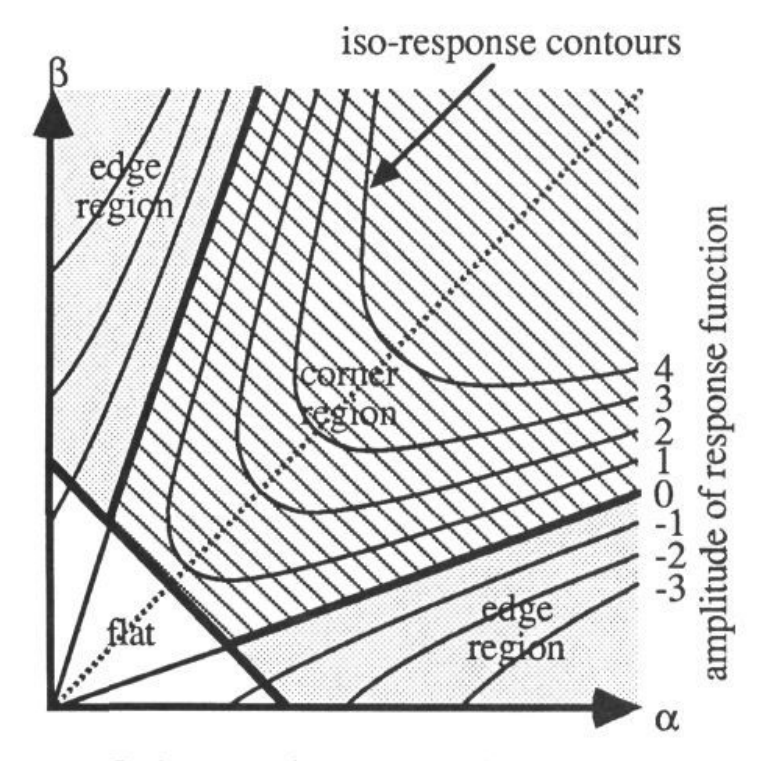
\includegraphics[width=0.6\linewidth]{structure_tensor.png}
    \caption{Visualisation of distinction of image features using the eigenvalues of the structure
        tensor~\cite{harris88}. $\alpha, \beta$ are equivalent to the eigenvalues $\lambda_1, \lambda_2$}\label{fig:Structure}
\end{figure}
\noindent There are several approaches to find out which case applies at the current position. The biggest
challenge here is to differentiate between edges and corners, i.e.\ we have to find out whether both
eigenvalues are meaningfully larger than 0 and if one is larger than the other.\\
The most intuitive approach is the one by Tomasi and Kanade~\cite{tomasi91}, sometimes also called Shi-Tomasi
corner detector. It simply compares the smaller eigenvalue against some artificial
threshold. The set of local maxima is then the set of corners for the image~\cite{shitomasi94}.
However, this approach requires to compute both eigenvalues and can thus be fairly expensive.
A cheaper approach would be to either threshold the trace 
\begin{equation}
    \tr(\mathbf{J}_\rho(\del\mathbf{u}_\sigma)) := j_{1, 1} + j_{2,
    2} = \lambda_1 + \lambda_2\label{def:Rohr}
\end{equation} 
as proposed by Rohr~\cite{rohr91} or the determinant 
\begin{equation}
    \det(\mathbf{J}_\rho(\del\mathbf{u}_\sigma)) := j_{1, 1}j_{2, 2} -
    j_{1, 2}^2 = \lambda_1\lambda_2\label{def:Harris}
\end{equation} 
as proposed by Harris~\cite{harris88} and Förstner~\cite{foerstner87}. Both of these approaches do 
not need to explicitly compute the eigenvalues of the structure tensor and are thus not as 
computationally expensive.\newpage\noindent
Another difference between both approaches is that~\eqref{def:Rohr} 
requires 
\begin{equation}
    \tr(\mathbf{J}_\rho(\del\mathbf{u}_\sigma))
\end{equation}
by itself to be a local maximum whereas in~\eqref{def:Harris}
\begin{equation}
    \frac{\det(\mathbf{J}_\rho(\del\mathbf{u}_\sigma))}{\tr(\mathbf{J}_\rho(\del\mathbf{u}_\sigma))}
\end{equation} 
needs to be a local maximum.\\
For the detection of relevant corners in the data selection phase, we mainly used the approach of
Förstner and Harris as well as
the approach of Rohr even though the Tomasi-Kanade approach was an option and has also been
tested as we will see later in Chapter~\ref{ch:Experiments}. However, it has not proven as successful
as the other two methods during the initial testing phase.
%%%%%%%%%%%%%%%%%%%%%%%%%%%%%%%%%%%%%  Diffusion %%%%%%%%%%%%%%%%%%%%%%%%%%%%%%%%%%%%%%%%%%%%%%
\section{Diffusion}\label{sec:Diffusion}
The concept of diffusion is omnipresent in the physical world. It describes, in the broadest sense
possible, how particles distribute in a certain medium. This could be anything from heat in air to
ink in water. But this is not its only use. It is applicable in many fields ranging from
natural sciences to finance and economics. In this chapter, we will see how diffusion applies to
image processing and what benefits we gain from it. Furthermore we will go over some basic ideas to
introduce diffusion mathematically and subsequently explain different types of diffusion commonly
found and used in image processing.
\subsection{A Short Note on Scale Spaces}\label{sub:ScaleSpaces}
Before we begin to talk about diffusion, we will use this opportunity to shortly introduce scale
spaces and explain how they are useful to diffusion processes in image processing and image
processing in general.\\
A scale space is generally defined as a family of images with a time parameter $t$ that become
increasingly `simpler' as $t \to \infty$. The point of a structure like this is that certain image
features do only exist at a specific scale or a range of scales and that it is therefore beneficial
to the understanding of an image to basically have a hierarchy of features~\cite{lindeberg94}.\\
Mathematically, a scale
space needs to meet certain requirements like the semi-group property, maximum-minimum principles
and others~\cite{weickert96, alvarez93}.\newpage\noindent
A full explanation of all the scale space requirements would be beyond the scope of this thesis
and is frankly not needed to understand the following sections.\\
To embed an image $f:\R^2 \rightarrow \R$ in a scale space, we need a smoothing
operator $T$ that is applied iteratively to the image. One such an operation is the Gaussian
convolution: 
\begin{equation}
    T_{t}f := K_{\sqrt{2t}} * f
\end{equation}
This operation spans the \textit{Gaussian scale space}, one of, if not the oldest and best
understood scale space. In the western world, it was first mentioned by Witkin~\cite{witkin84} in 1984,
but as was later found out and published in~\cite{weickert-ishikawa}, it was already derived
axiomatically by Japanese researcher Taizo Ijima in 1959~\cite{ijima}. \\
Scale spaces as a tool are very important to diffusion filtering, since diffusion is an iterative
process and as such benefits from the notion of a scale spaces. Embedding an image in such a scale
space allows us to develop a theory of evolving the image over time as we will see in the next
sections, where we first motivate the idea behind the general diffusion equation and
subsequently introduce different types of diffusion important to image processing.
To avoid confusion we define the gradient for scale spaces as the \textit{spatial gradient} 
\begin{equation}
    \del \mathbf{u}(x, y, t) = \begin{pmatrix}
        \partial_x u(x, y, t)\\
        \partial_y u(x, y, t)
    \end{pmatrix} 
\end{equation}
instead of the spatiotemporal gradient.

\subsection{Mathematical Background}
To get a glimpse of the basic idea of diffusion, we have to take a small dive into the world of
physics.
As mentioned in the introduction to this section, diffusion is used to describe processes of
particle or concentration distribution. The differences in concentration are evened out by a flow
or \textit{flux} that is aimed from high concentration areas to areas with low concentration. This
principle is stated by \textit{Fick's law}~\eqref{eq:Fick} (hence this type of diffusion is called \textit{Fickian
diffusion}):
\begin{equation}
    \boldsymbol j = -\boldsymbol D\cdot\del \mathbf{u}\label{eq:Fick}
\end{equation}
Here, the flow from high to low concentration areas is modelled by a flow whose direction is
proportional to the inverse direction of the largest change in concentration, i.e.\ the gradient.
While most of the time, the gradient determines the direction of the flux, the so called
\textit{diffusion tensor} $\boldsymbol D$ determines its strength. \\

\noindent In general, this diffusion
tensor is defined as a
$2\times2$ positive definite matrix, but as we will see later, it can be reduced to a scalar 
valued function in more simple cases.
In more complex cases, also called \textit{anisotropic}, the diffusion tensor can also adjust the
direction of the flow. We will see how this works in the section about \textit{nonlinear
anisotropic diffusion}.\\
Another important principle for diffusion is the conservation of mass, stating that mass can neither be
created nor destroyed.
This principle is given by the equation
\begin{equation}
    \partial_t u = - \textnormal{div}(\boldsymbol j)\label{eq:Conservation}
\end{equation}
where $u: \Omega \times [0, \infty) \rightarrow \R$ is a function of time and space and div
is the \textit{divergence operator}
\begin{equation}
    \textnormal{div}(\boldsymbol j) := \partial_x j_1 + \partial_y j_2
\end{equation}
In simple terms, the divergence of the flux measures whether the concentration at the current
location diverges, i.e.\ diffuses away from the current location, or converges, i.e.\ moves in
towards the current location.
\begin{figure}[H]
    \centering
    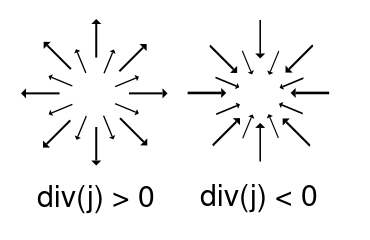
\includegraphics[width=0.5\linewidth]{divergence2.png}
    \caption{Visualisation of the divergence operator~\cite{img-divergence}. Original image edited
    with GIMP~\cite{gimp}}\label{fig:Divergence}
\end{figure}
\noindent Together, equations~\eqref{eq:Fick} and~\eqref{eq:Conservation} then form the general \textit{diffusion
    equation}~\cite{dic, weickert96}
\begin{equation}
    \partial_t u = \textnormal{div}(\boldsymbol D\cdot\del \mathbf{u})\label{eq:Diffusion}
\end{equation}
The solution to this equation can be interpreted as an image embedded in a scale space with the
evolution time as the scale parameter. To get different scale spaces ergo different diffusion
processes, one can alter the diffusion tensor in certain ways.
In the following, we will see how different diffusion processes are characterized and what they are
generally most useful for in image processing.

\subsection{Isotropic Diffusion}
\subsubsection*{Linear isotropic diffusion}
In this first and simplest case, the diffusion tensor is replaced by a constant diffusivity
resulting in equal smoothing all across the image. The constant diffusivity can also be expressed
as the identity matrix $\boldsymbol I$ which simplifies the diffusion equation to the 2D\textit{
heat equation}
\begin{equation}
    \partial_t u = \Delta u = \textnormal{div}(\del \mathbf{u})\label{eq:IsoDiff}
\end{equation}
which can be solved analytically. The solution to this equation has proven to be equivalent to
a Gaussian convolution, thus this type of diffusion also produces a Gaussian scale space.\\
Obviously, homogeneous smoothing is not very useful if one wants to create a filter that is able to
enhance edges. Still, it is the best understood and oldest scale space and used for many
applications in image processing. One example is optical character recognition.
However, to achieve edge enhancing properties, we need to look into nonlinear methods.

\subsubsection*{Nonlinear isotropic diffusion}\label{sub:NonIsoDiff}
Previously, we replaced the diffusion tensor by the identity matrix, which resulted in the same
amount of smoothing at every location.
To get spatially varying smoothing, we have to introduce a \textit{diffusivity} function that
depends continuously on the input image. 
\begin{align}
    \boldsymbol D &= g(\lVert\del \mathbf{u}\rVert_2^2)\boldsymbol I\\
    \Rightarrow \partial_t u & = \textnormal{div}(g(\lVert\del
    u\rVert_2^2)\del \mathbf{u})\label{eq:NonIsoDiff}
\end{align}
The diffusivity function determines how much the image should be smoothed at the current location.
The most well known choice for a diffusivity function was proposed by Perona and Malik 
~\cite{perona-malik}
\begin{equation}
    g(s^2) = \frac{1}{1 + s^2/\lambda^2}\label{def:Diffusivity}
\end{equation}
The interesting part about this diffusivity function is that it distinguishes between edges and
non-edges or flat areas according to the \textit{contrast parameter} $\lambda$ using the gradient
magnitude $\lVert\del \mathbf{u}\rVert_2^2$ as a \textit{fuzzy edge detector}~\cite{dic}. \\
\\ \\ 
\noindent An important part of understanding why this leads to an edge enhancing effect is the flux function
arising from this specific diffusivity. In general, the flux function is simply defined as 
\begin{equation}
    \Phi(s) = sg(s^2)
\end{equation}
which in this particular case comes down to
\begin{equation}
    \Phi(s) =\frac{s}{1 + s^2/\lambda^2}\label{def:Flux}
\end{equation}
\begin{figure}
    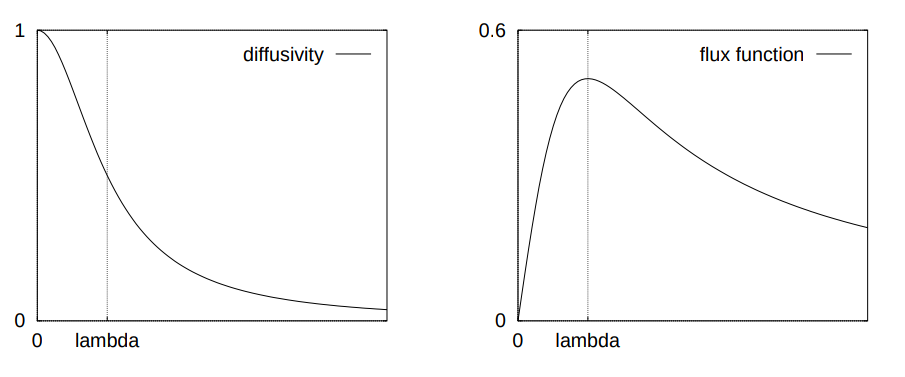
\includegraphics[width=\linewidth]{diffflux.png}
    \caption{\textbf{Left:} Diffusivity mentioned in~\eqref{def:Diffusivity}. \textbf{Right:} Flux
    function~\eqref{def:Flux}~\cite{dic}.}\label{fig:DiffFlux}
\end{figure}
As we already know, the flux describes the change in concentration at each position. The edge
enhancing effect comes from the so called \textit{backwards diffusion} which happens when the
gradient magnitude surpasses the contrast parameter as seen in Figure~\ref{fig:DiffFlux}. Backwards
diffusion is basically the opposite from `normal' diffusion in a sense that it sharpens image
features instead of smoothing them.
If we look at the derivative of the flux function this will become more obvious:
\begin{equation}
    \Phi'(s) = \frac{d}{ds} \left(\frac{s}{1 + s^2/\lambda^2}\right) = 
    \frac{1 - s^2/\lambda^2}{{\left(1 + s^2/\lambda^2\right)}^2}
\end{equation}
As we see, we have a maximum in the flux function at $s = \lambda$. Furthermore we can extract from
the above equation that $\Phi'(s) < 0$ for $s < \lambda$ and $\Phi'(s) > 0$ for $s > \lambda$. This
can also be seen in Figure~\ref{fig:DiffFlux}. This distinction between an increasing and decreasing flux
function for values left and right from the contrast parameter causes the previously mentioned
edge enhancing effect.\newpage\noindent
However, this particular process is not \textit{well-posed}~\cite{weickert96}, i.e.\ it is very
sensitive to high frequent noise. To solve this, it was proposed to use Gaussian smoothing for
\textit{regularisation}, that means to convolve the original image with a Gaussian kernel to damp the high
frequencies that cause numerical instabilities~\cite{catte-lions-morel92}.

\subsection{Anisotropic Diffusion}
However, we can still go one step further and even make the direction of the smoothing process dependent
on the local structure. For example, one might want to prevent smoothing across edges and rather
smooth parallel to them further embracing the edge-preserving nature of nonlinear diffusion.\\
The diffusion tensor in this case is constructed from its eigenvectors $\boldsymbol v_1,
\boldsymbol v_2$ and eigenvalues $\lambda_1, \lambda_2$ using the
theorem of matrix diagonalisation
\begin{equation}\label{eq:DiffTensor}
    \boldsymbol D = \left(\boldsymbol v_1\vert \boldsymbol v_2\right) \textnormal{diag}(\lambda_1, \lambda_2)
    \begin{pmatrix}
        \boldsymbol v_1^\top\\
        \boldsymbol v_2^\top
    \end{pmatrix}
\end{equation}
We define the eigenvectors to be
\begin{equation}
    \boldsymbol v_1 = \del \mathbf{u}_\sigma,\qquad\boldsymbol v_2 = \del \mathbf{u}_\sigma^\bot
\end{equation}
As mentioned before, we want to encourage smoothing along edges and in flat regions. Thus, we
define the eigenvalue for the eigenvector parallel to the gradient to be 1 and the eigenvalue to
the orthogonal one to be a diffusivity function similar to the one in the nonlinear isotropic case.
\begin{equation}
    \lambda_1 = g(\lVert\del \mathbf{u}_\sigma\rVert_2^2),\qquad\lambda_2 = 1
\end{equation}
There are different viable choices for a diffusivity function that supports backwards diffusion.
Firstly, there is the already mentioned Perona-Malik diffusivity~\eqref{def:Diffusivity}. Another
option is the diffusivity function introduced by Weickert~\cite{weickert96}
\begin{equation}
    g(s^2) = \begin{cases}
        1 & s^2 = 0\\
        1 - \exp\left(\frac{-3.31488}{{(s/\lambda)}^8}\right) & s^2 > 0
    \end{cases}\label{def:WeickertDiff}
\end{equation}
According to~\cite{dic}, diffusivities of this type, i.e.\ rapidly decreasing diffusivities,
lead to more segmentation-like results.
Finally, the diffusivity that was mainly used for inpainting in this work is the
\textit{Charbonnier diffusivity}~\cite{charbonnier}
\begin{equation}
    g(s^2) = \frac{1}{\sqrt{1 + s^2 / \lambda^2}}\label{def:CharbonnierDiff}
\end{equation}
\begin{figure}[H]
    \centering
    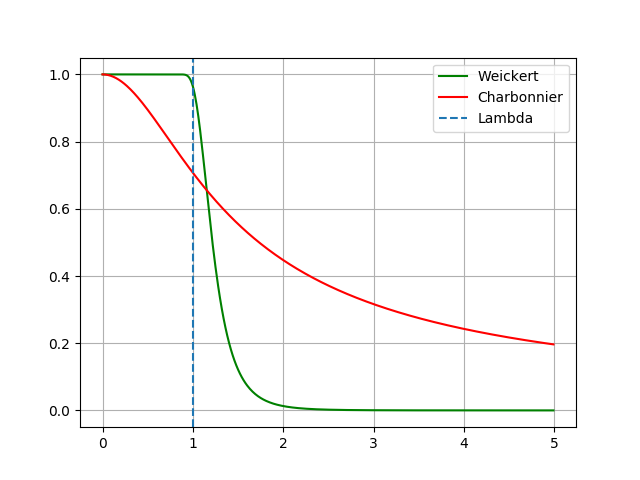
\includegraphics[width=\linewidth]{diffusivities.png}
    \caption{Weickert~\eqref{def:WeickertDiff} and Charbonnier~\eqref{def:CharbonnierDiff}
    diffusivities for $\lambda = 1$. Graph created with Matplotlib~\cite{matplotlib}}
\end{figure}
\noindent Overall, we can write the EED equation as
\begin{equation}
    \partial_t u = \diverg(g(\del \mathbf{u}_\sigma\del \mathbf{u}_\sigma^\bot)\del \mathbf{u})\label{def:EED}
\end{equation}
As we see in figure~\ref{fig:DiffExamples}, EED possesses great restoration and denoising
capabilities. Nonetheless, as already mentioned in Related Work (\ref{ch:RelatedWork}), edge-enhancing
diffusion is not
only suited for image denoising~\cite{galic05, weickert96}, but also one of the best methods for inpainting based on partial
differential equations~\cite{galic08, schmaltz09, schmaltz14}.
\begin{figure}[H]
    \centering
    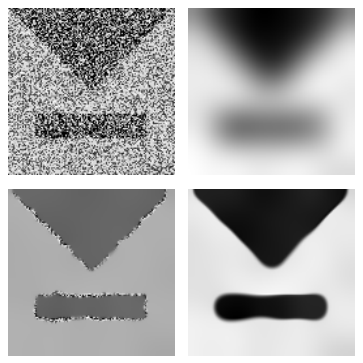
\includegraphics[width=0.8\linewidth]{diff_examples.png}
    \caption{Denoising capabilities of the different types of diffusion~\cite{weickert96}. \textbf{Top Left:} Original
        image. \textbf{Top Right:} Linear isotropic diffusion. \textbf{Bottom Left:} Nonlinear
    isotropic diffusion. \textbf{Bottom Right:} Edge-enhancing diffusion.}\label{fig:DiffExamples}
\end{figure}

\section{Inpainting}\label{sec:Inpainting}
Inpainting itself originated as a technique used by image restorators and conservators and has
been in use for many decades, centuries even. The main objective of inpainting is
to restore damaged regions in an image or even filling in areas that are missing
completely. In the analog or physical world, inpainting is often done in multiple steps as
described in~\cite{bertalmio00}:\\
Firstly, the lines defining the structure surrounding the blank area are continued inside the area.
The smaller areas that result by drawing in the structure lines are then filled in with colours that
match the colours outside the blank area.
Lastly, texture and small details are added.\\
Since this obviously cannot be applied to digital images, people had to come up with a way to
translate this process to the digital domain.

\subsection{The Origin of Digital Inpainting}
In 2000, Bertalmio et al.~\cite{bertalmio00} proposed a method to digitize this inpainting
technique.
Together with Masnou and Morel~\cite{masnou98}, this was one of the first attempts to come up 
with a digital image inpainting algorithm.
The idea behind their algorithm was to iteratively continue so called \textit{isophote
lines}, i.e.\ lines of equal brightness, inside the missing areas. 
This was implemented by an image evolution described by 
\begin{equation}
    \partial_t u = \mathbf{\nabla_n} L(u)  
\end{equation}
where $L(u) = \diverg(\del \mathbf{u}) = u_{xx} + u_{yy}$ and $\nabla_\mathbf{n}$ is the 
directional derivative in the direction $n$. Note that in this particular case, the evolution is
only performed in the inpainting regions. The regions of the image that are already known, are left
unprocessed. The direction $\mathbf{n}$ is given by the vector
\begin{equation}
    \mathbf{n} = {(\del \mathbf{u})}^\bot = \begin{pmatrix}
        u_y\\-u_x
    \end{pmatrix}
\end{equation}
which is orthogonal to the image gradient $\del \mathbf{u}$ as defined in~\ref{def:Grad}.
The formula can also be written as 
\begin{equation}
    \partial_t u = \langle \del L(u), \del \mathbf{u}^\bot\rangle
\end{equation}
The evolution given by this formula basically propagates information from outside of the blank
area along the direction of isophote lines arriving at the boundary of this area, conserving the
angle of arrival between the boundary and the isophote line~\cite{bertalmio00}.
This direction is given by a vector orthogonal to the gradient, i.e.\ the direction of the largest
grey value change.
Why this is the case becomes more obvious if we restate this to say that a vector orthogonal to the gradient
determines the direction of the \textit{smallest} grey value change, which ultimately is the
direction of a line of equal brightness.\\
This propagation is then complemented by a (\textit{anisotropic}) diffusion process that is performed regularly to
\textit{periodically curve the lines to keep them from crossing each other}~\cite{bertalmio00}.
By alternatingly applying the prolongation and diffusion process, the inpainting regions are
shrinked progressively until they vanish as can be seen in~\ref{fig:InpaintingProgress}.
\begin{figure}[h]
    \centering
    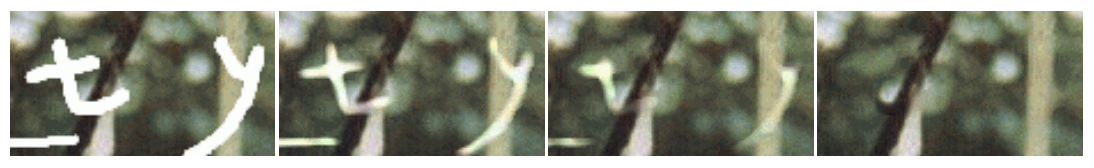
\includegraphics[width=\linewidth]{inpainting_progress.png}
    \caption{Results of the inpainting process at different stages showing the progressive
    shrinking of the inpainting regions~\cite{bertalmio00}.}\label{fig:InpaintingProgress}
\end{figure}
\newpage\noindent
\subsection{EED-based Inpainting}\label{sub:EEDInpaint}
The general idea behind inpainting methods based on partial differential equations  is to
retrieve an image in the form of an unknown function $v: \Omega \rightarrow \R$ as described 
in~\cite{galic05}. Let $\Omega_1\subset\Omega$ be the subset of locations where the values 
of $v$ are known from the original image. The \textit{inpainting domain}, that is the locations 
where we want to reconstruct the image, is then given as the set $\Omega\backslash\Omega_1$. 
The goal is now to find a sufficiently often continuously differentiable function
$u:\Omega\rightarrow\R$ that satisfies
\begin{equation}
    u(x) = v(x)\quad\forall x\in\Omega_1
\end{equation}
Moreover, we want $u$ to be sufficiently \textit{close} to $f$ in $\Omega\backslash\Omega_1$.\\
The idea to find such a function is to specify an image evolution which yields the desired
function as its \textit{steady state}, i.e.\ a state where $\partial_{t}u = 0$. More intuitively 
steady state means that the function does not evolve any further with increasing $t$ once it has
reached this state.\\
Generally, the evolution for a PDE-based inpainting problem is given by
\begin{equation}
    \partial_t u(x,t) = (1-c(x))Lu(x,t) - c(x) (u(x, t) - f(x))\label{eq:Evolution}
\end{equation}
where 
\begin{equation} 
    c(x) := \begin{cases}
        1&x\in\Omega_1\\
        0&\text{elsewhere}
    \end{cases} 
\end{equation}
is the characteristic function of the subset $\Omega_1$ and $f:\Omega\rightarrow\R$ is the
initial state of the evolution given by
\begin{equation} 
    f(x) := \begin{cases}
        v(x)&x\in\Omega_1\\
        0&\text{elsewhere}
    \end{cases} 
\end{equation}
\newpage\noindent
On the boundary $\partial\Omega$ of the image domain, homogeneous Neumann boundary conditions are
applied, which can be expressed mathematically as 
\begin{equation*}
    \partial_\mathbf{n}u = \langle \mathbf{n}, \del \mathbf{u} \rangle = 0
\end{equation*}
where $ \mathbf{n}$ is the normal vector to the image boundary.
The so called \textit{steady state equation}
\begin{align}
    (1 - c(x))Lu(x,t)- c(x)(u(x, t) - f(x)) = 0\label{eq:SteadyState}
\end{align}
determines the behaviour of the evolution as $t\to\infty$ and therefore defines the desired
function $u$. Namely, for $x\in\Omega_1$,~\eqref{eq:SteadyState} implies that 
\[ u(x,t) = f(x) \]
by using $c(x) = 1$ and similarly we get for $x\in\Omega\backslash\Omega_1$, that $c(x) = 0$ and
thus
\[ Lu(x, t) = 0 \]
Using this, one can rewrite the original equation~\eqref{eq:Evolution} in a simpler way by
introducing \textit{Dirichlet boundary conditions} given by the subset $\Omega_1$ of known values on the 
inpainting domain and solving the evolution equation
\begin{equation}
    \partial_t u(x,t) = Lu(x, t)
\end{equation}
The choice of the differential operator $L$ is still an active topic of
research, but it was shown in~\cite{schmaltz14} that edge-enhancing diffusion~\eqref{def:EED} is the best choice
among those tested.
The authors' explanation of the `favourable' performance of this operator in the context of
inpainting is, that the inherent anisotropic behaviour of the operator allows it to create sharp
edges while still being able to propagate directional information to outside of the known area.
They explain this ability to propagate information by the Gaussian smoothing that is found in the
definition of the diffusion tensor~\eqref{eq:DiffTensor}.
Other candidates that were being tested in~\cite{schmaltz14} include the \textit{biharmonic
and triharmonic operator} respectively defined as
\begin{eqnarray*}
    Lu = -\Delta^2u\\
    Lu = \Delta^3u
\end{eqnarray*}
a nonlinear isotropic diffusion operator as described in~\eqref{eq:NonIsoDiff} and simple
homogeneous diffusion~\eqref{eq:IsoDiff}.\newpage\noindent
In Figure~\ref{fig:DiffOpsCompare}, (f) and (e) refer to the nonlinear isotropic diffusion defined
in~\eqref{eq:NonIsoDiff} and the regularised version also mentioned in~\ref{sub:NonIsoDiff}.
\begin{figure}[h]
    \centering
    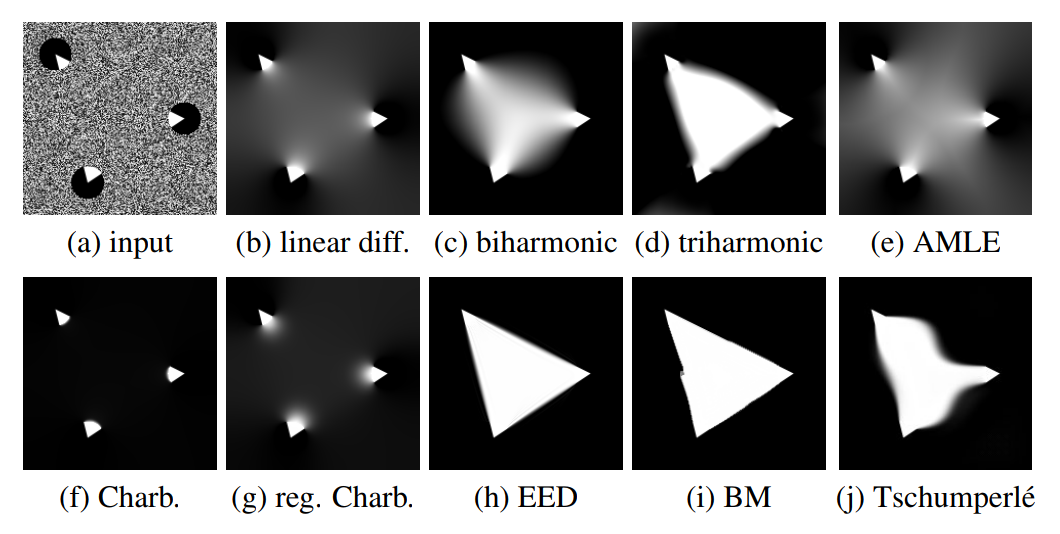
\includegraphics[width=\linewidth]{diffops_compare.png}
    \caption{Comparison of different differential operators for PDE-based
    inpainting~\cite{schmaltz14}.}\label{fig:DiffOpsCompare}
\end{figure}
